\section{Zdefiniowanie interfejsów do prezentacji, edycji i obsługi danych\\
Zdefiniowanie panelu sterowania aplikacji}
Poniżej prezentujemy zrzuty ekranu prezentujące funkcjonalność (wraz z numerem odpowiedniej funkcji)
\begin{figure}[!htp]
    \centering
    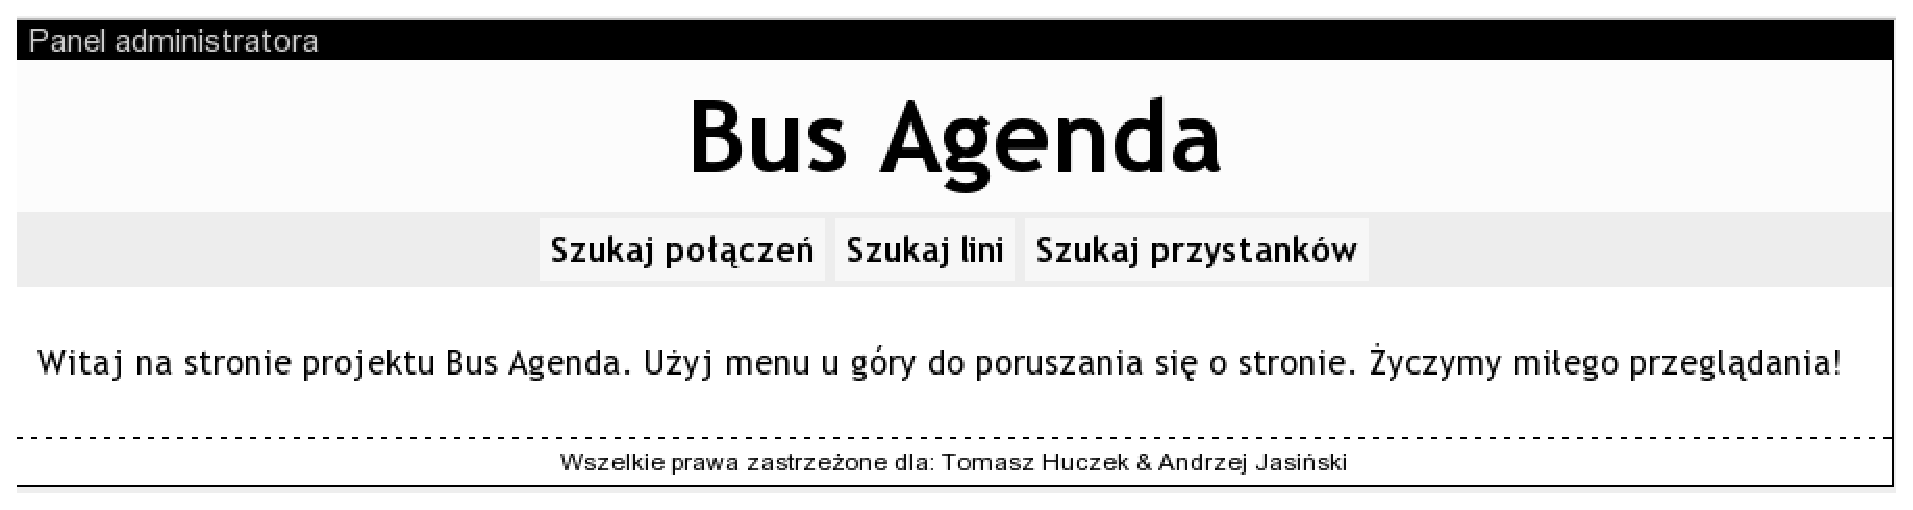
\includegraphics[width=0.8\textwidth]{./img/screens/mainScreen.eps}
    \caption{Główne okno aplikacji - domyślnie jako użytkownik (Funkcja 2)}
    \label{fig:main}
\end{figure}

\begin{figure}[!htp]
    \centering
    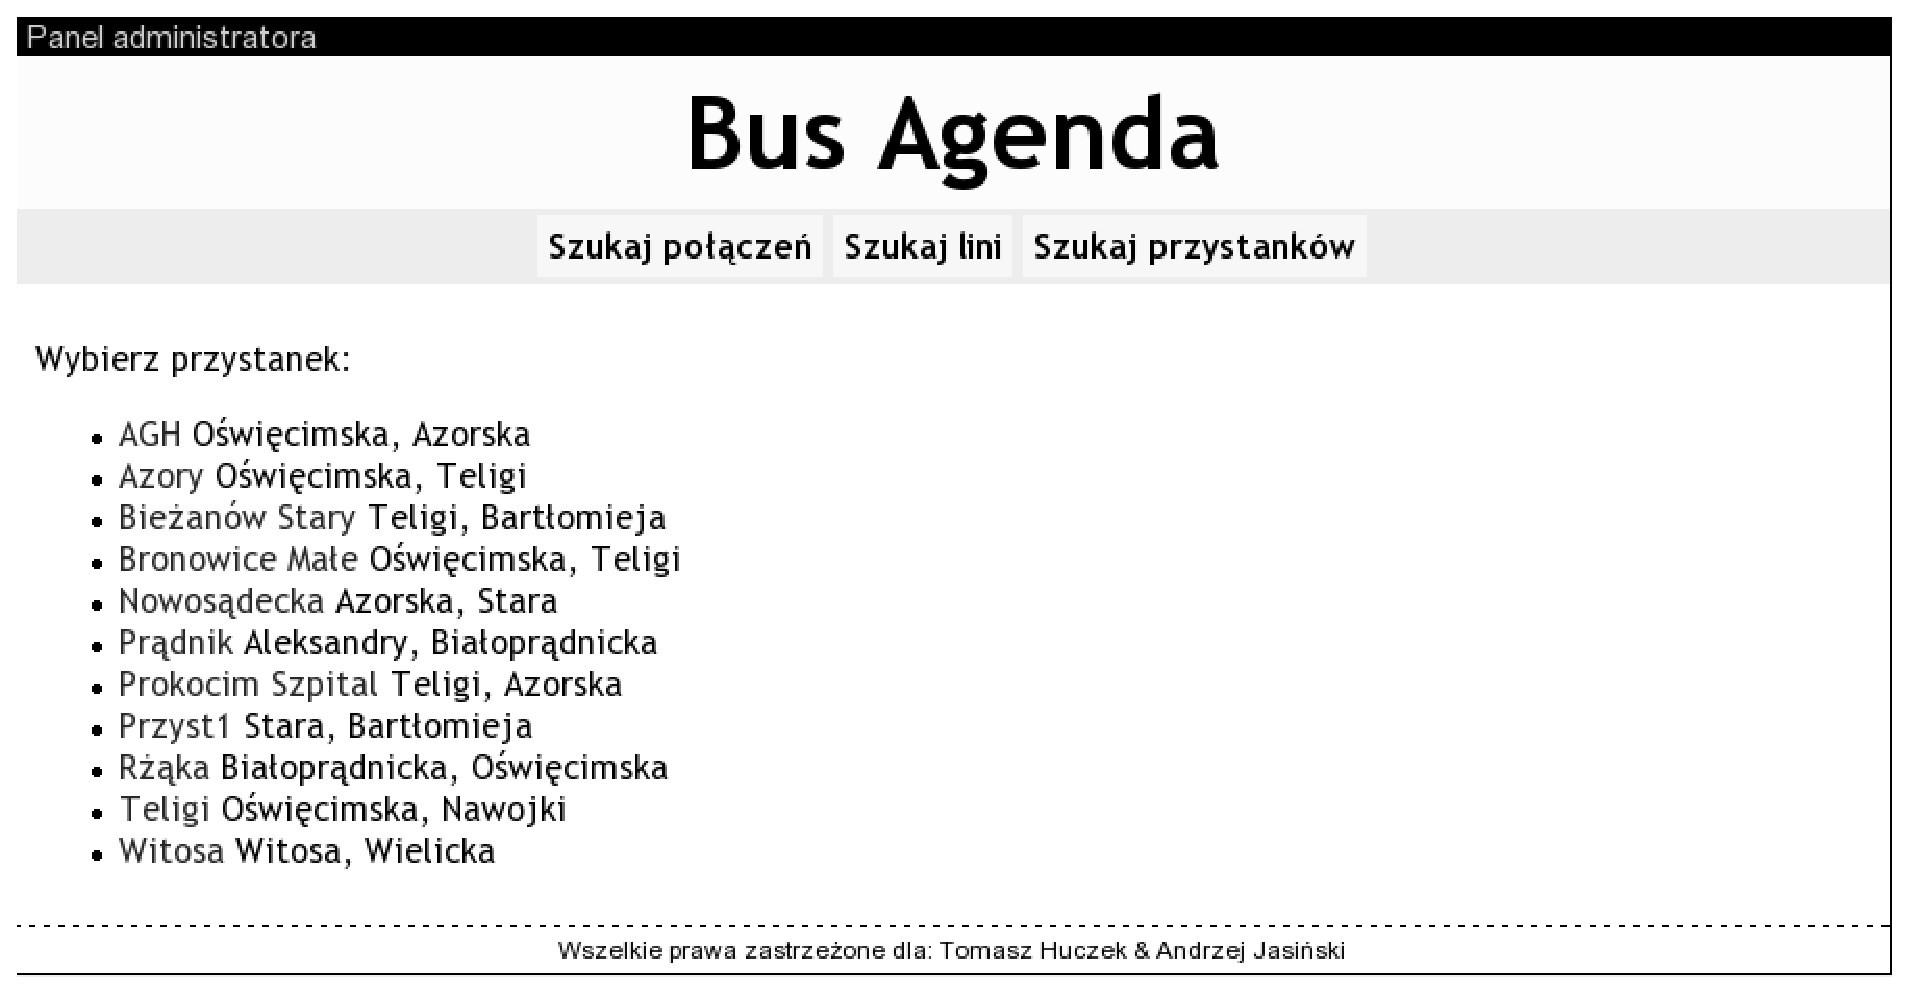
\includegraphics[width=0.8\textwidth]{./img/screens/BusStopsSearch.eps}
    \caption{Ekran poszukiwania przystanków (Funkcja 2.1.3)}
    \label{fig:searchBS}
\end{figure}

\begin{figure}[!htp]
    \centering
    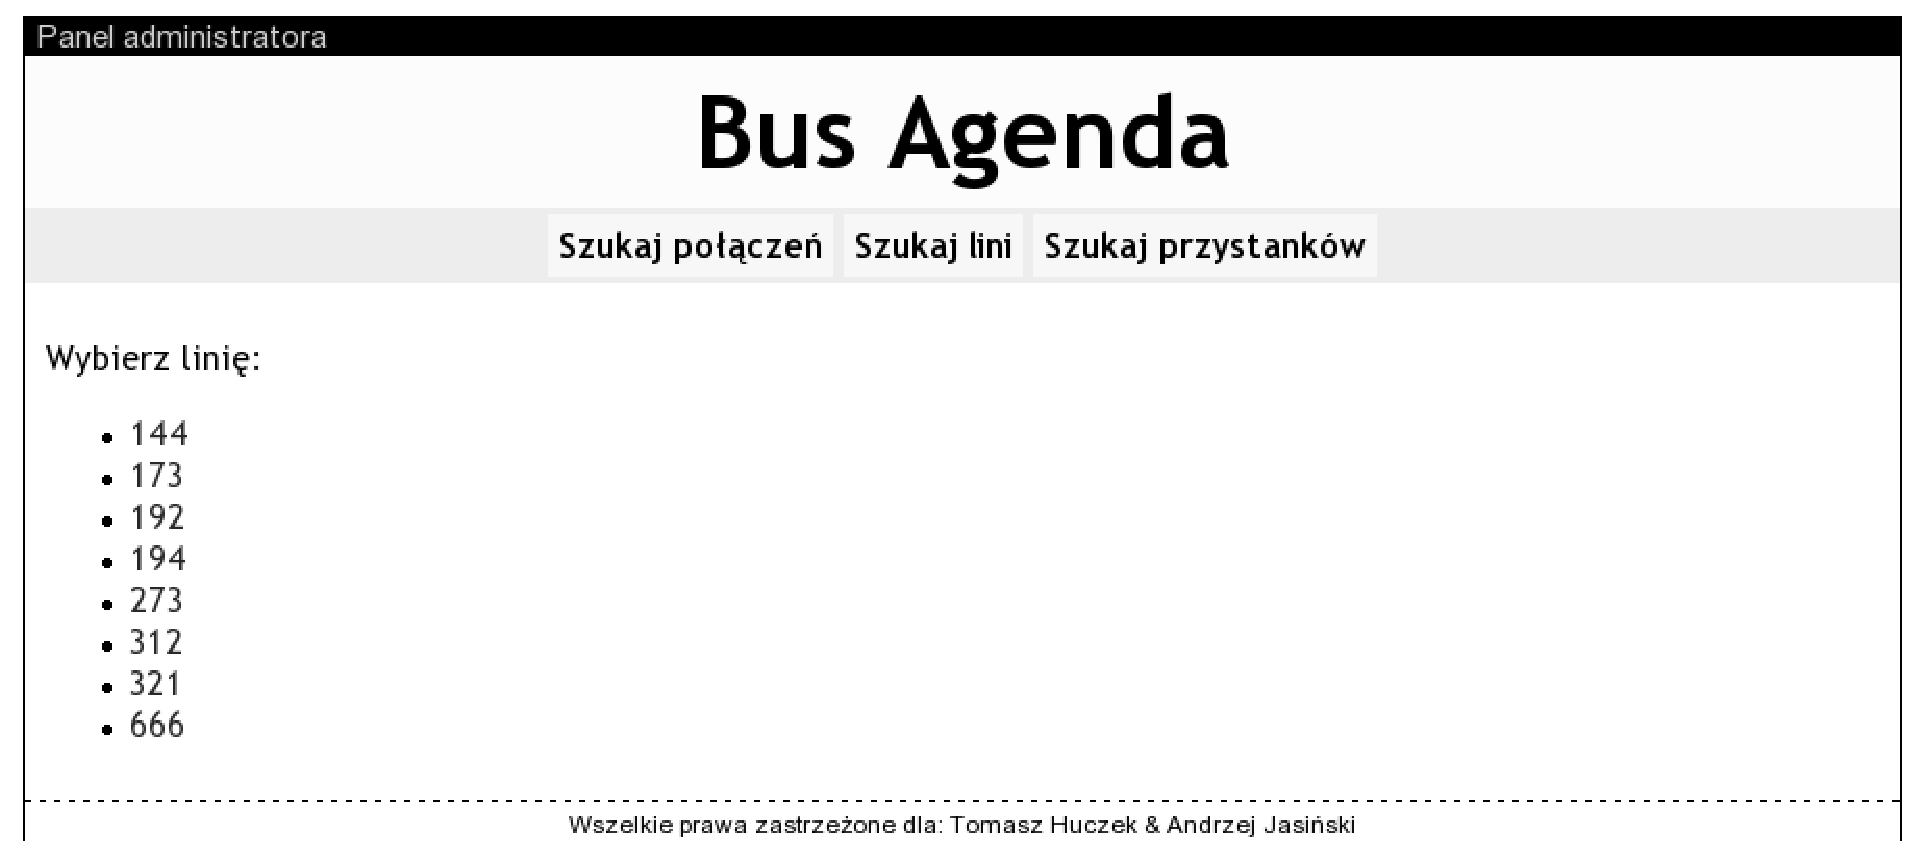
\includegraphics[width=0.8\textwidth]{./img/screens/linesSearch.eps}
    \caption{Ekran poszukiwnania linii (Funkcja 2.1.2)}
    \label{fig:searchLine}
\end{figure}

\begin{figure}[!htp]
    \centering
    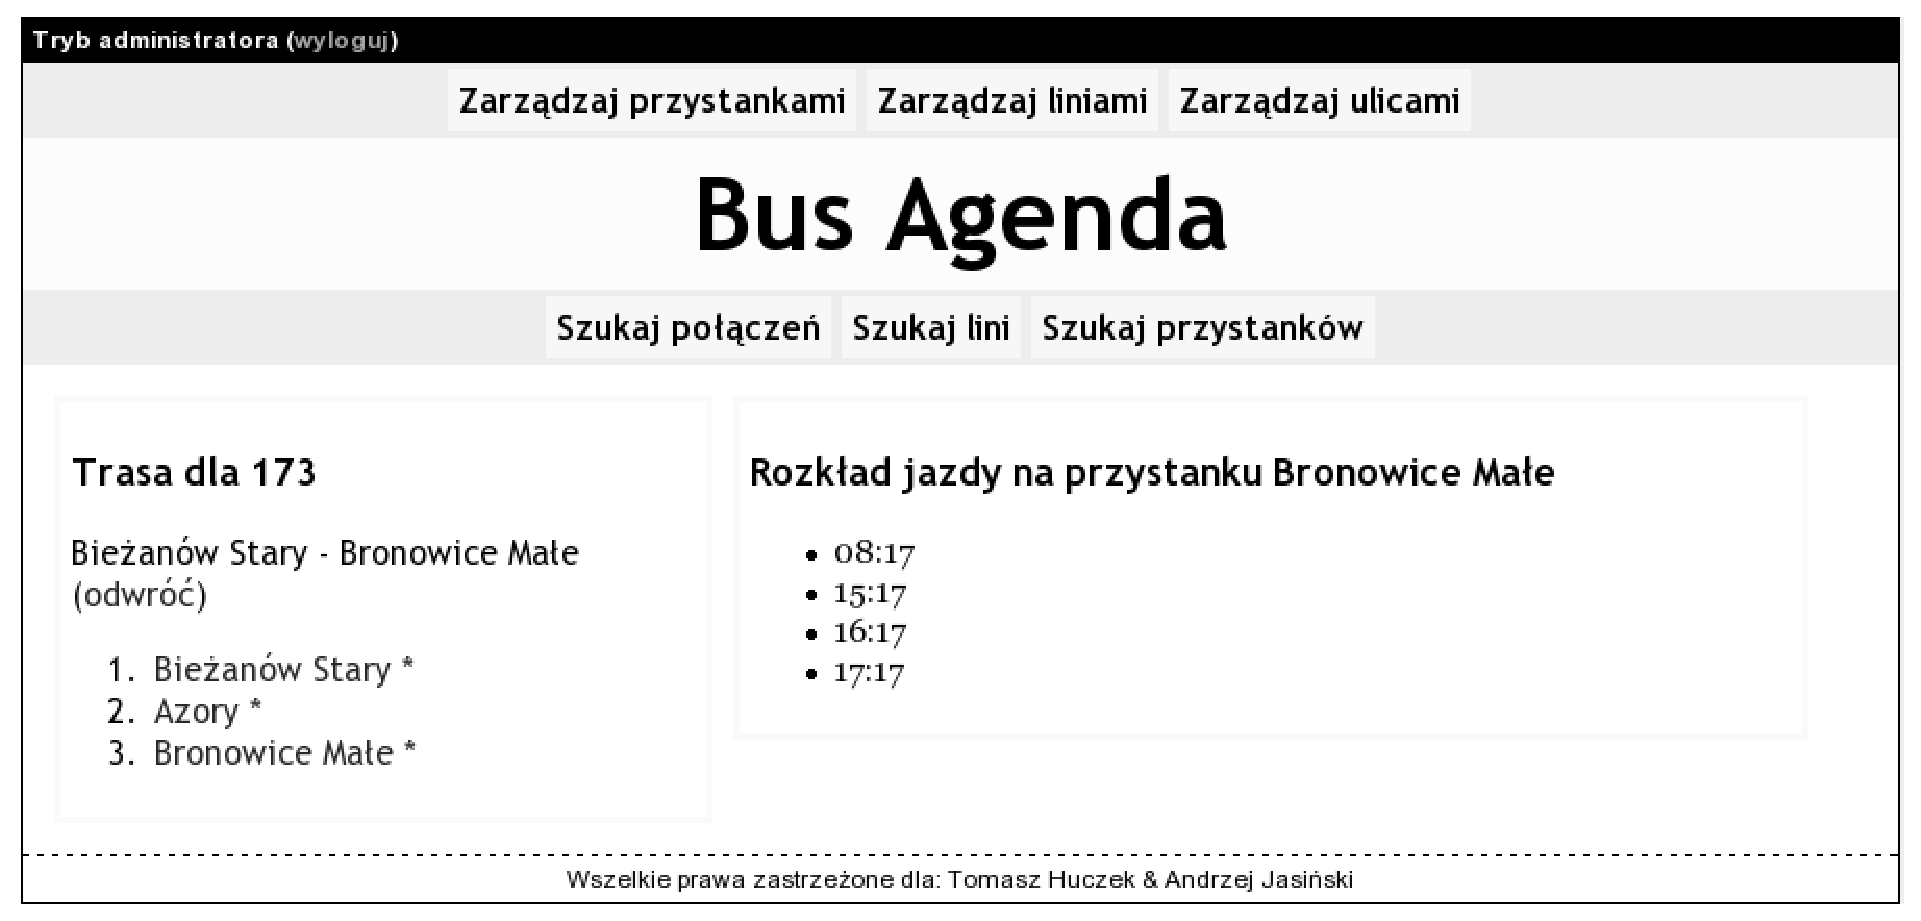
\includegraphics[width=0.8\textwidth]{./img/screens/showTT.eps}
    \caption{Oglądanie rozkładu (Funkcja 2.1.4)}
    \label{fig:showTT}
\end{figure}

\begin{figure}[!htp]
    \centering
    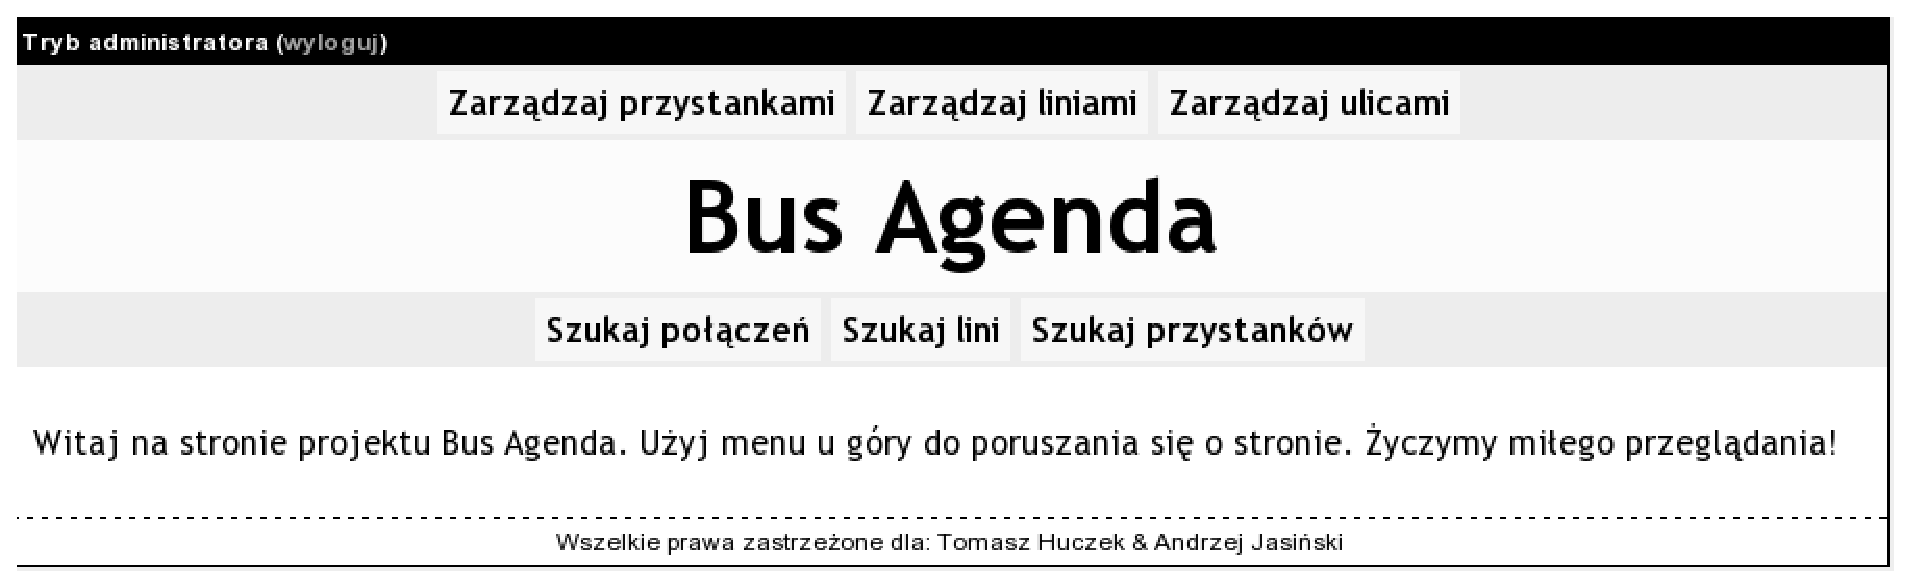
\includegraphics[width=0.8\textwidth]{./img/screens/adminMain.eps}
    \caption{Panel administratora (Funkcja 1)}
    \label{fig:adminMain}
\end{figure}
%
\begin{figure}[!htp]
    \centering
    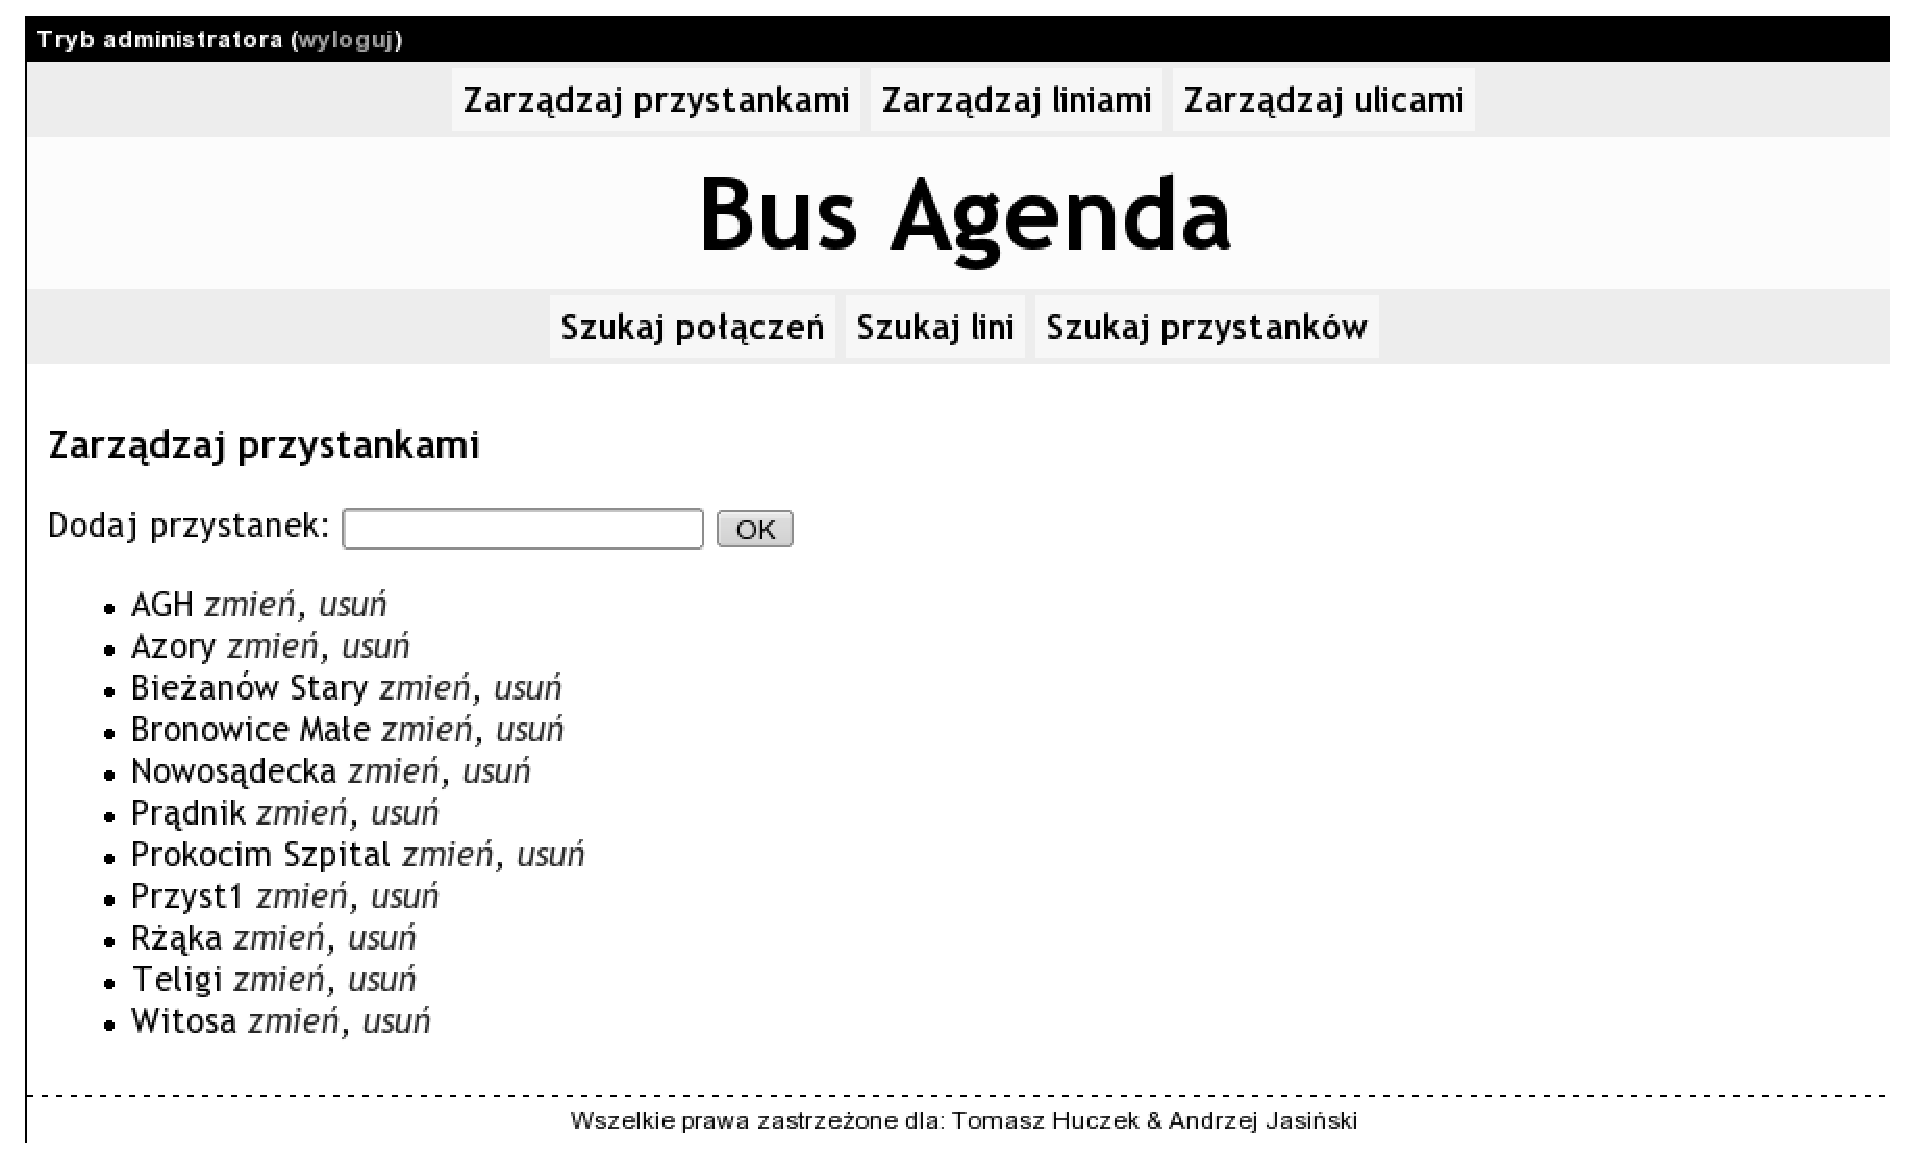
\includegraphics[width=0.8\textwidth]{./img/screens/manageBS_main.eps}
    \caption{Zarządzanie przystankami (Funkcja 1.2 oraz 1.2.1 i 1.2.3)}
    \label{fig:adminMain}
\end{figure}
\begin{figure}[!htp]
    \centering
    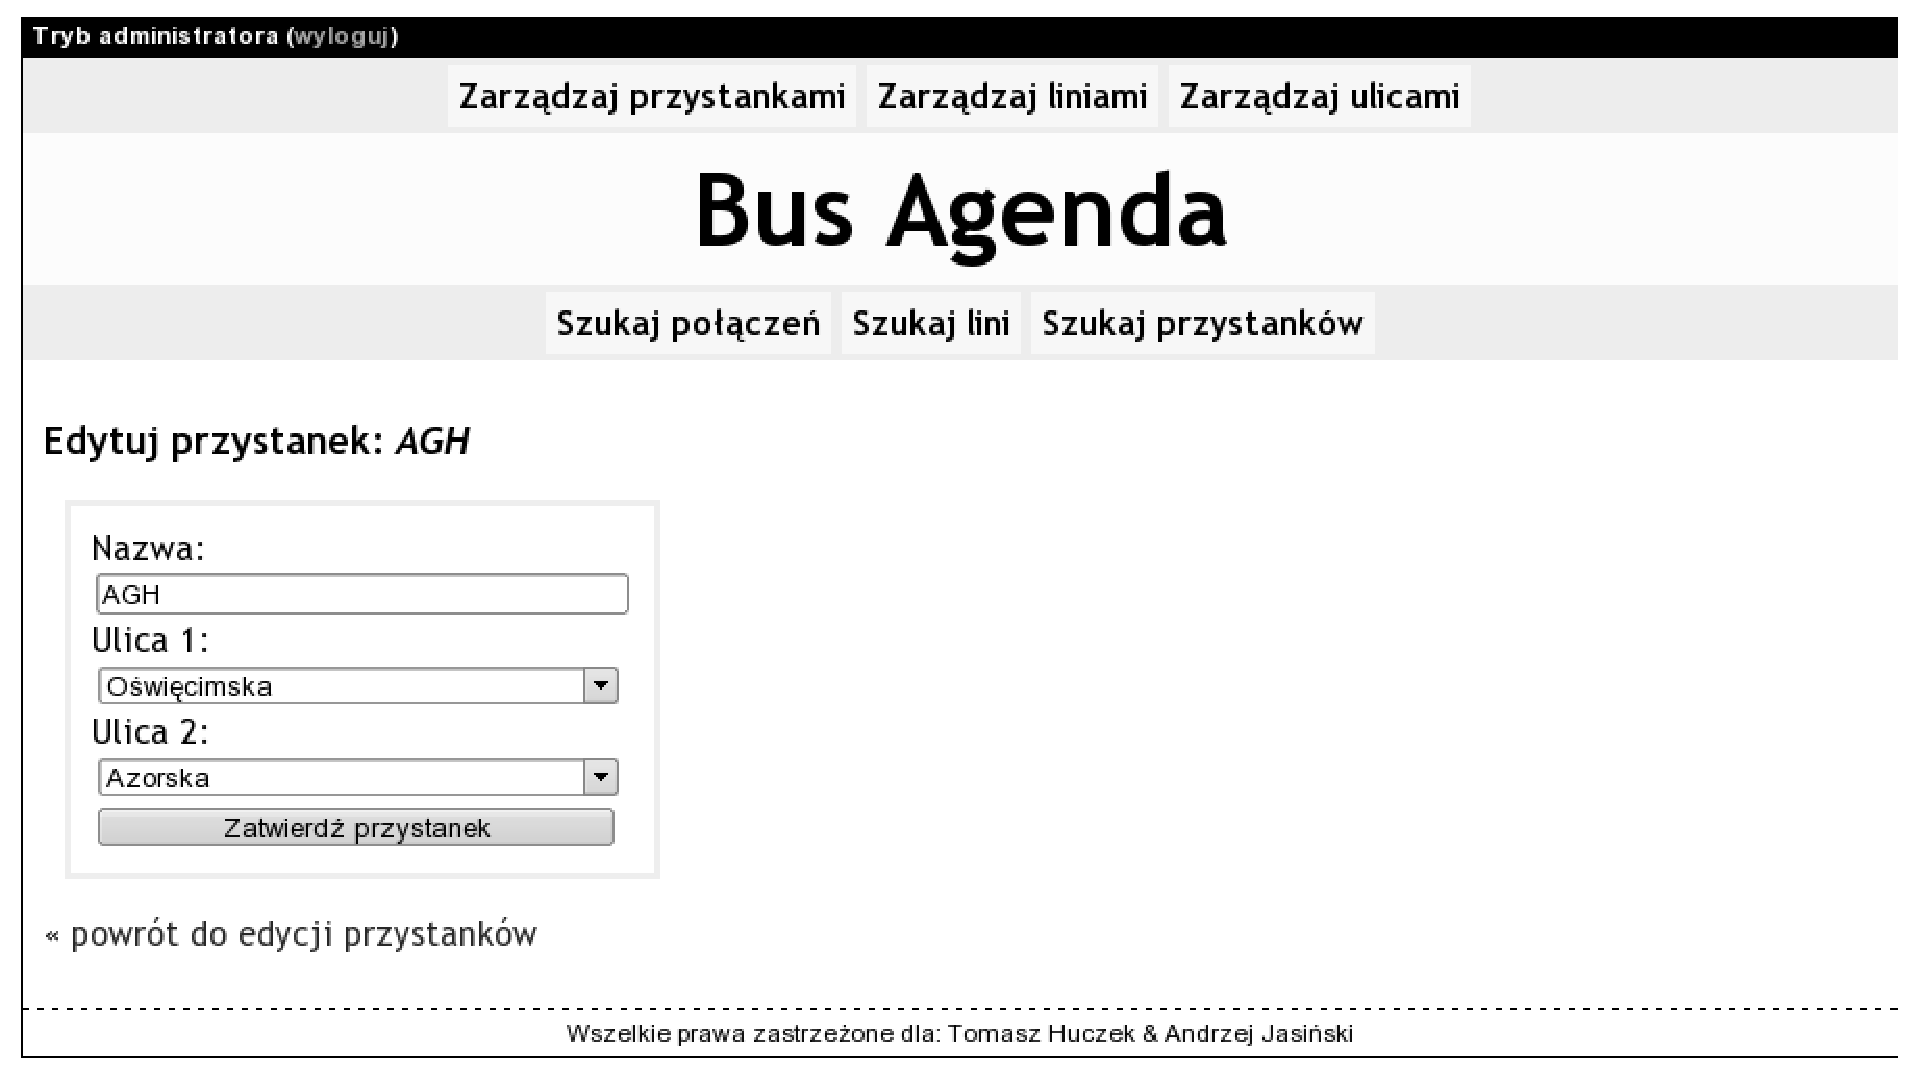
\includegraphics[width=0.8\textwidth]{./img/screens/manageBS.eps}
    \caption{Edycja przystanku (Funkcja 1.2.2)}
    \label{fig:adminMain}
\end{figure}
\begin{figure}[!htp]
    \centering
    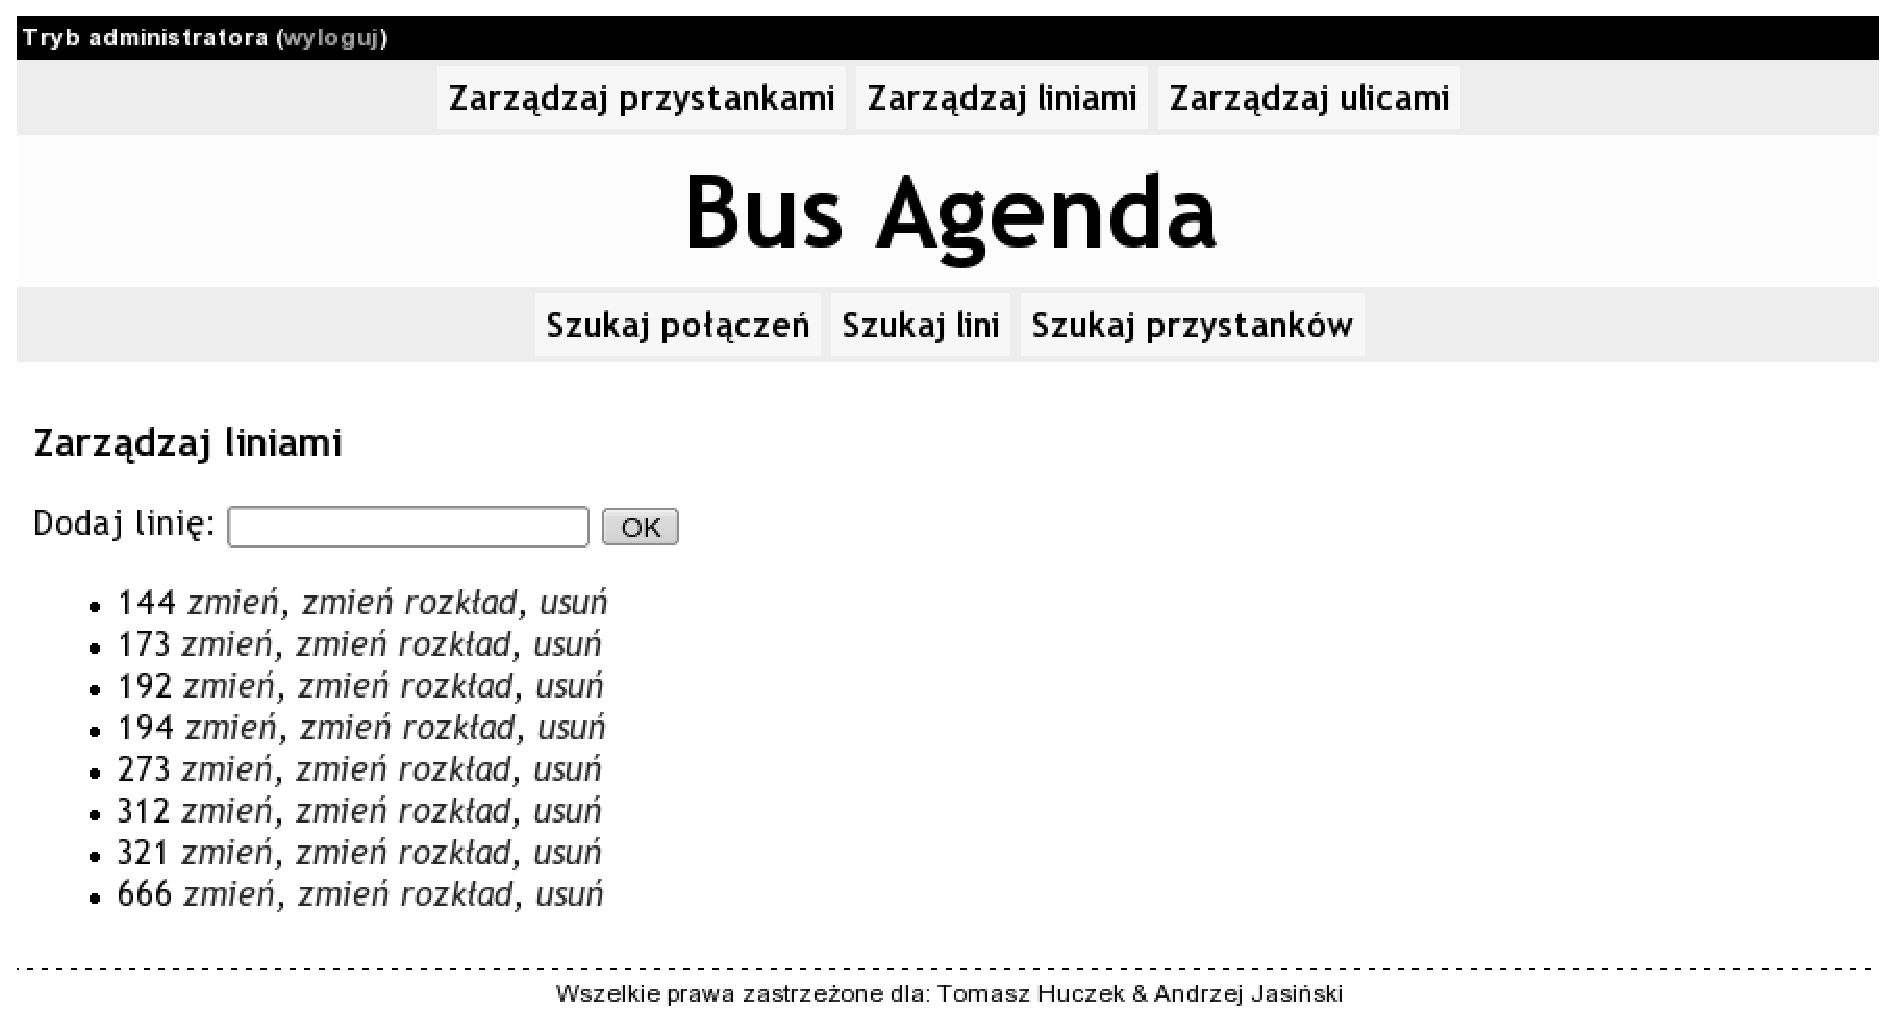
\includegraphics[width=0.8\textwidth]{./img/screens/manageLines_main.eps}
    \caption{Zarządzanie liniami (Funkcja 1.1 oraz 1.1.1 i 1.1.2)}
    \label{fig:adminMain}
\end{figure}
\begin{figure}[!htp]
    \centering
    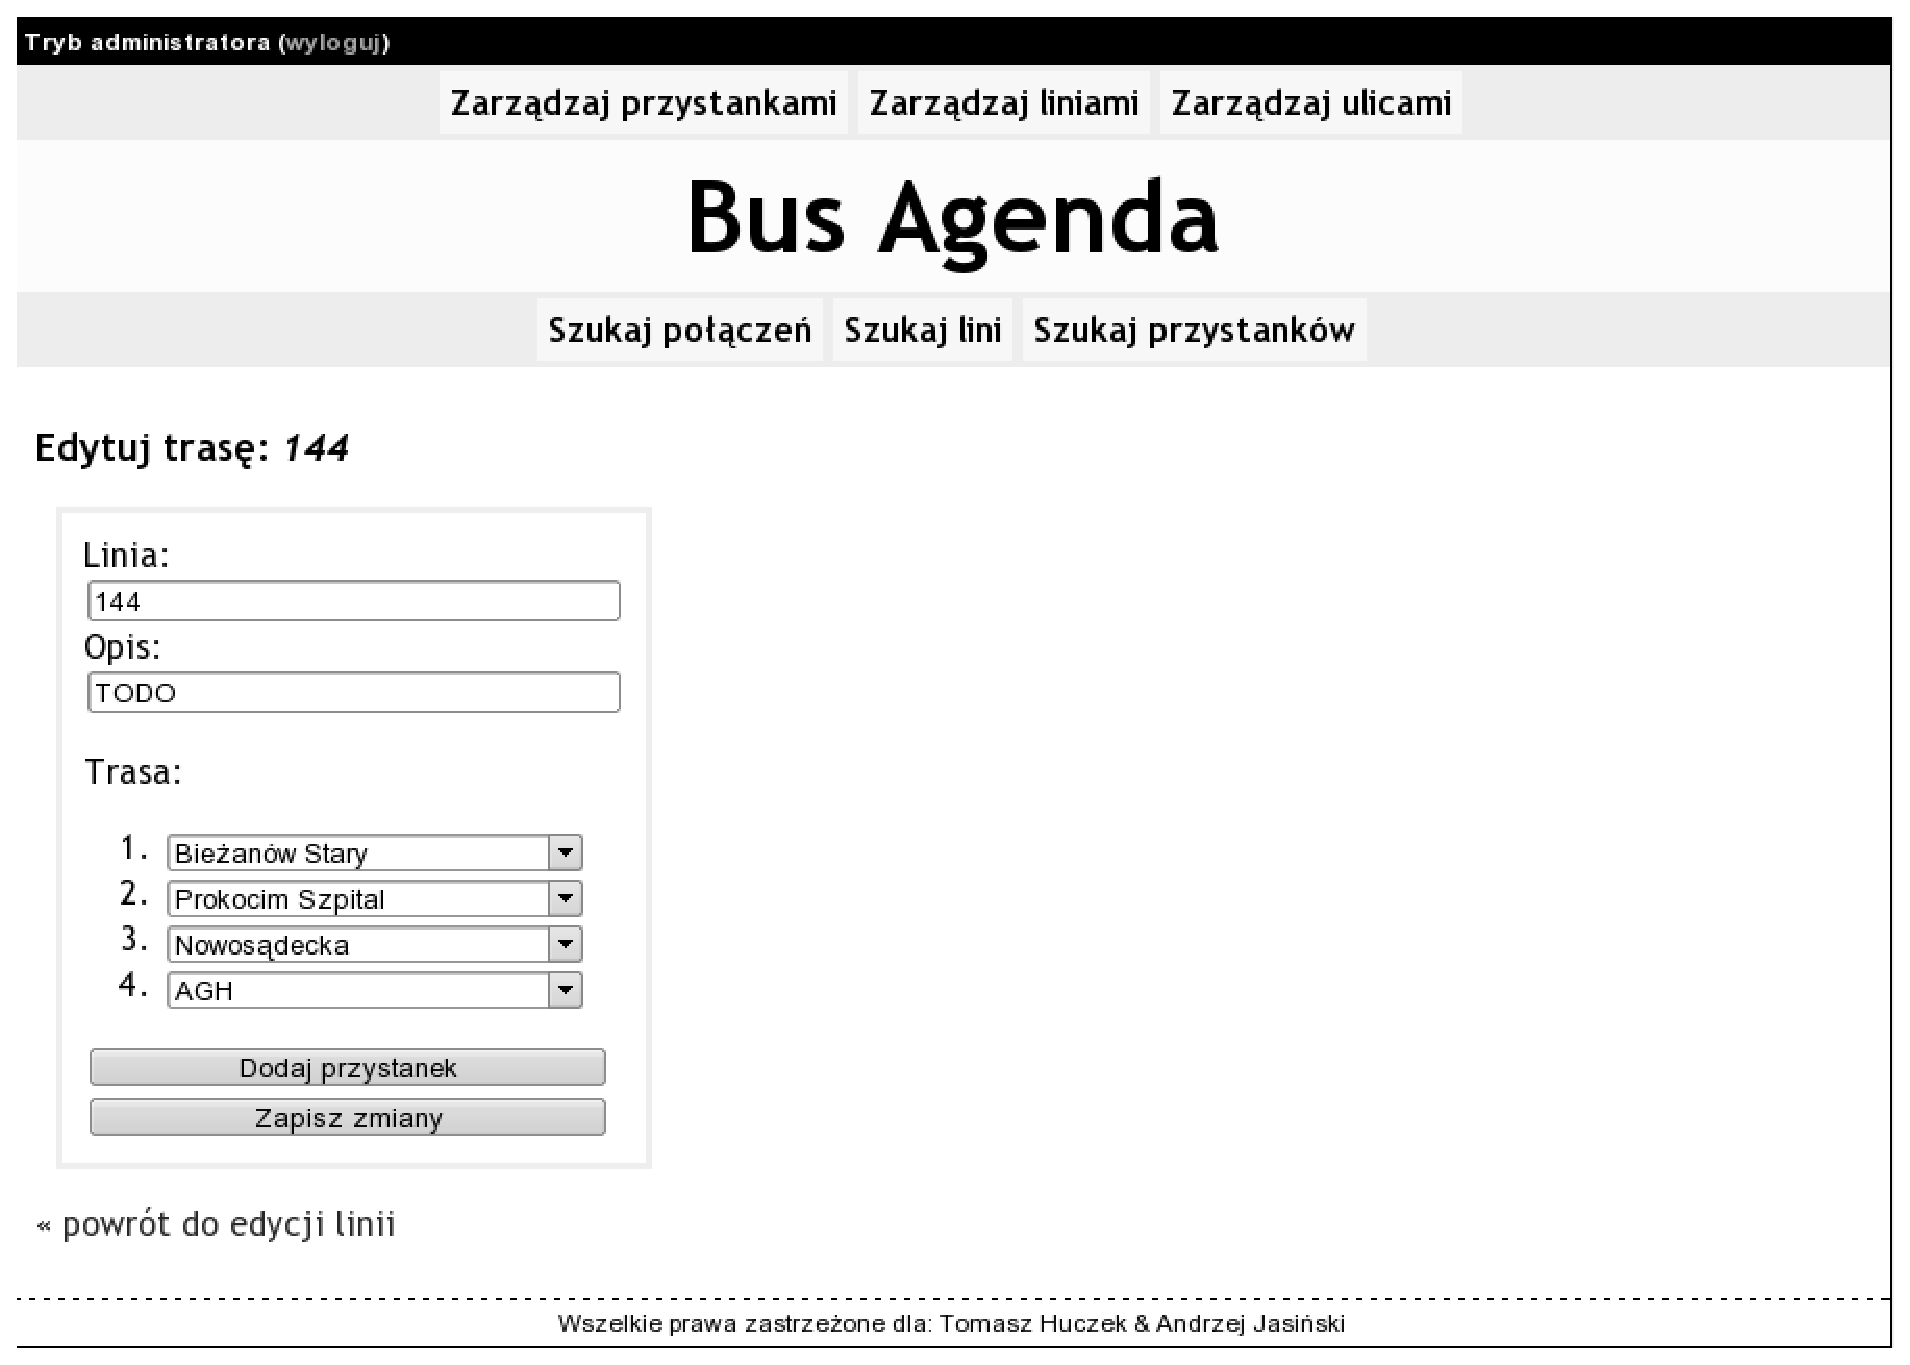
\includegraphics[width=0.8\textwidth]{./img/screens/manageLine.eps}
    \caption{Edycja linii (Funkcja 1.1.3)}
    \label{fig:adminMain}
\end{figure}
\begin{figure}[!htp]
    \centering
    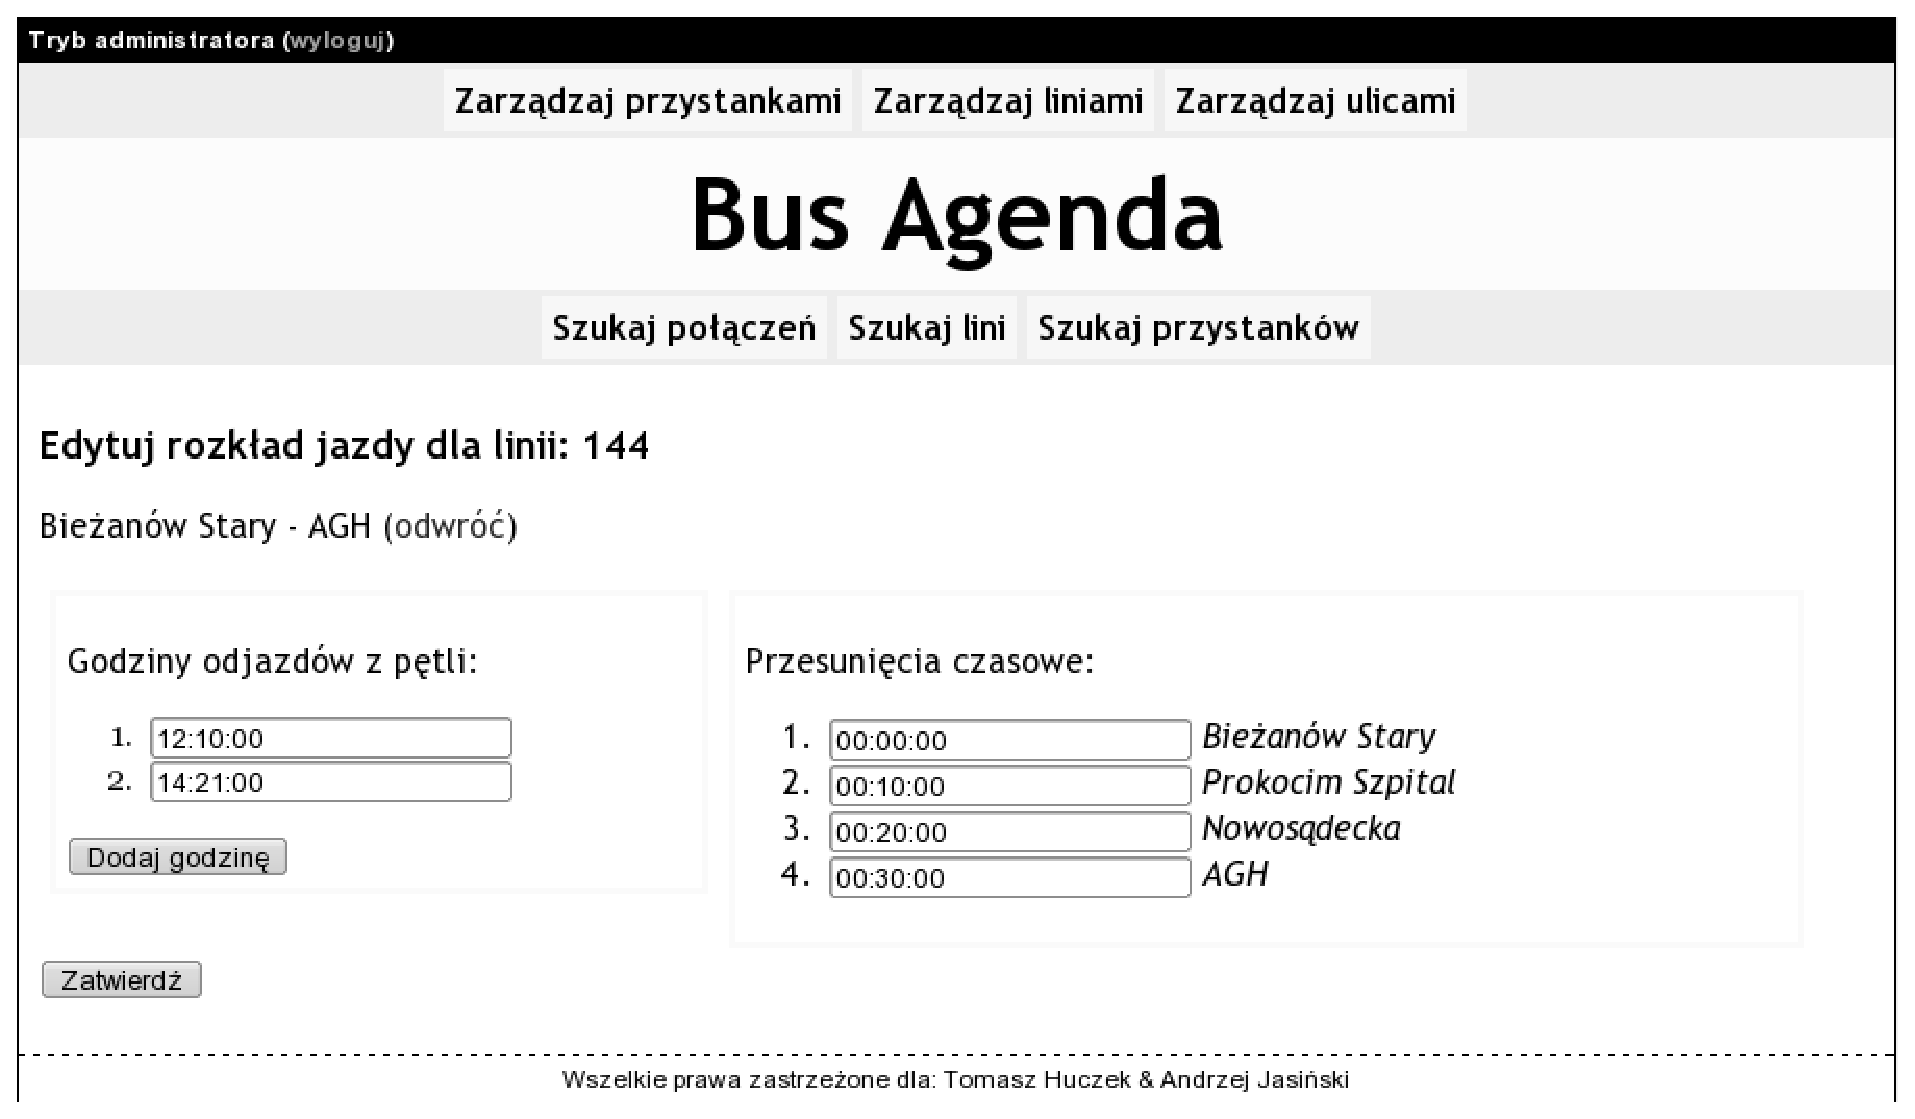
\includegraphics[width=0.8\textwidth]{./img/screens/manageLine_tt.eps}
    \caption{Zmień rozkład danej linii (Funkcja 1.1.3.1)}
    \label{fig:adminMain}
\end{figure}
\begin{figure}[!htp]
    \centering
    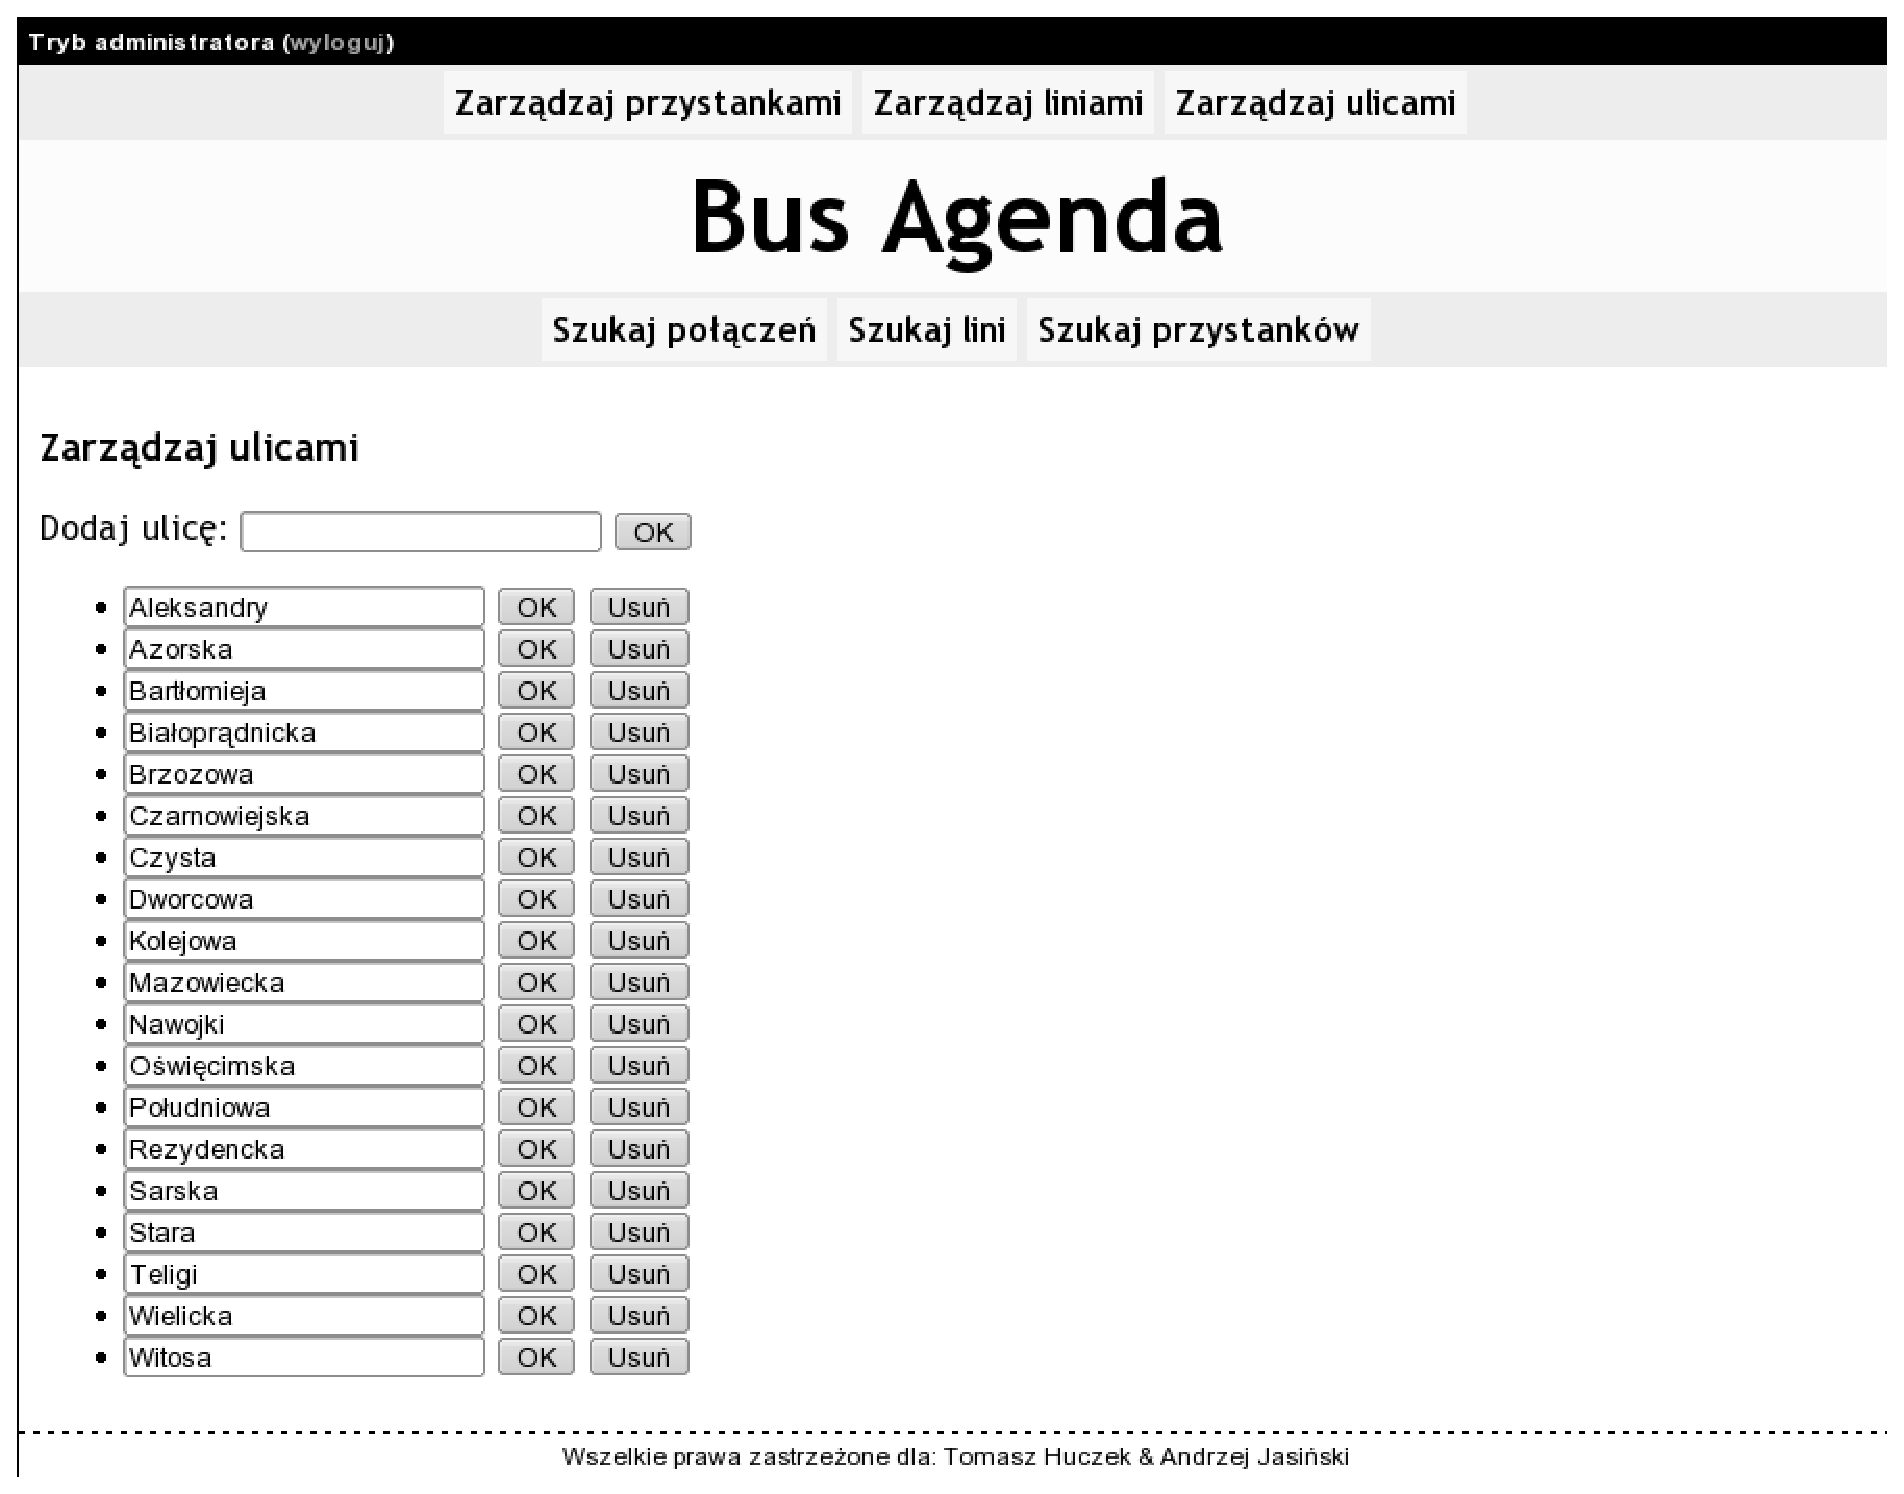
\includegraphics[width=0.8\textwidth]{./img/screens/manageStreets_main.eps}
    \caption{Zarządzanie ulicami (Funkcja 1)}
    \label{fig:adminMain}
\end{figure}